\documentclass[a4paper,12pt,fleqn]{article}

\usepackage{amsmath}
\usepackage[margin=1in]{geometry}
\usepackage{xcolor}
\usepackage{tikz}
\usepackage{subcaption}
\usepackage[hypertexnames=false,bookmarksnumbered=true,final]{hyperref}
\usepackage[capitalize,sort]{cleveref}
\usetikzlibrary{decorations.pathreplacing,arrows.meta,calc,3d,perspective}

\def\colorschemesepia{sepia}
\def\colorschemedark{dark}
\def\colorschemelight{light}

\ifx\colorscheme\undefined
\let\colorscheme\colorschemelight
\fi

\ifx\colorscheme\colorschemelight
\colorlet{textColor}{black}
\colorlet{bgColor}{white}
\fi

\ifx\colorscheme\colorschemesepia
\definecolor{textColor}{HTML}{433423}
\definecolor{bgColor}{HTML}{fbf0da}
\fi

\ifx\colorscheme\colorschemedark
\definecolor{textColor}{HTML}{bdc1c6}
\definecolor{bgColor}{HTML}{202124}
\colorlet{textHeavy}{white}
\definecolor{textRed}{HTML}{ff968c}  % hsb(5 deg, 45%, 100%)
\definecolor{textGreen}{HTML}{70cc70}  % hsb(120 deg, 45%, 80%)
\definecolor{textBlue}{HTML}{8cbcff}  % hsb(215 deg, 45%, 100%)
\definecolor{textCyan}{HTML}{70cccc}  % hsb(180 deg, 45%, 80%)
\definecolor{textMagenta}{HTML}{d982d9}  % hsb(300 deg, 40%, 85%)
\definecolor{textYellow}{HTML}{bfbf69}  % hsb(60 deg, 45%, 75%)
\else
\colorlet{textHeavy}{black}
\colorlet{textRed}{red!50!black}
\colorlet{textGreen}{green!50!black}
\colorlet{textBlue}{blue!50!black}
\colorlet{textCyan}{cyan!80!black}
\colorlet{textMagenta}{magenta!80!black}
\colorlet{textYellow}{yellow!60!black}
\definecolor{textPurple}{HTML}{681da8}
\fi

\colorlet{dimColor}{textColor!50!bgColor}

\ifx\colorscheme\colorschemelight\else
\pagecolor{bgColor}
\color{textColor}
\fi

%\hypersetup{colorlinks,linkcolor=textRed,citecolor=textRed,urlcolor=textBlue}

\hypersetup{colorlinks,linkcolor=textRed,citecolor=textRed,urlcolor=textBlue}

\DeclareMathOperator{\opt}{opt}
\let\eps\varepsilon

\title{Bin Packing}
\author{\empty}
\date{\empty}

\begin{document}

\maketitle
\setlength{\parskip}{0.5em}

\section{Introduction}

In the classical bin packing problem, we are given a set $I$ of items.
Each item $i \in I$ has a size $s(i) \in (0, 1]$ associated with it.
Our goal is to partition $I$ into the minimum number of bins,
such that the sum of sizes of items in each bin is at most 1.
See \cref{fig:1bp} for an example.
The classical bin packing problem and its generalizations
have diverse applications in computer science and operations research,
like packing goods into trucks, allocating jobs to servers,
allocating memory in computers~\cite{handbook-of-combinopt-bp},
or assigning advertisements to station breaks in television programming.

\begin{figure}[!ht]
\centering
\begin{subfigure}{0.9\textwidth}
    \centering
    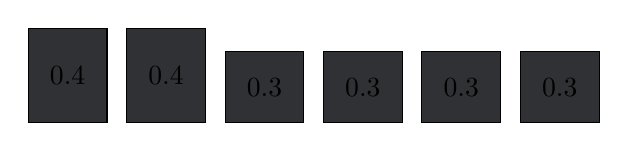
\begin{tikzpicture}[item/.style={fill={textColor!10!bgColor},draw}]
\path[item]
    (0,0) rectangle +(1,1.2) node[pos=0.5] {0.4}
    ++(1.25,0) rectangle +(1,1.2) node[pos=0.5] {0.4}
    ++(1.25,0) rectangle +(1,0.9) node[pos=0.5] {0.3}
    ++(1.25,0) rectangle +(1,0.9) node[pos=0.5] {0.3}
    ++(1.25,0) rectangle +(1,0.9) node[pos=0.5] {0.3}
    ++(1.25,0) rectangle +(1,0.9) node[pos=0.5] {0.3};
\end{tikzpicture}

    \caption{A set of six items: two items have size 0.4 and four items have size 0.3.}%
\label{fig:1bp:a}
\end{subfigure}
\par\bigskip\bigskip
\begin{subfigure}{0.45\textwidth}
    \centering
    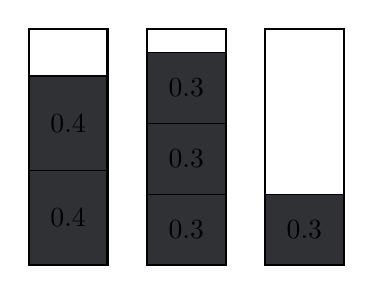
\begin{tikzpicture}[
item/.style={fill={textColor!10!bgColor},draw},
bin/.style={draw,thick},
]
\path[item]
    (0.0,0.0) rectangle +(1,1.2) node[pos=0.5] {0.4}
    (0.0,1.2) rectangle +(1,1.2) node[pos=0.5] {0.4}
    (1.5,0.0) rectangle +(1,0.9) node[pos=0.5] {0.3}
    (1.5,0.9) rectangle +(1,0.9) node[pos=0.5] {0.3}
    (1.5,1.8) rectangle +(1,0.9) node[pos=0.5] {0.3}
    (3.0,0.0) rectangle +(1,0.9) node[pos=0.5] {0.3};
\path[bin]
    (0,0) rectangle +(1,3)
    ++(1.5,0) rectangle +(1,3)
    ++(1.5,0) rectangle +(1,3);
\end{tikzpicture}

    \caption{A packing of the items into 3 bins.}
\end{subfigure}
\begin{subfigure}{0.45\textwidth}
    \centering
    \input{img/1bp-c.tikz}
    \caption{A packing of the items into 2 bins.}
\end{subfigure}
\caption[An example of classical bin packing.]{An example of classical bin packing.
We want to minimize the number of bins, so the packing into 2 bins
is better than the packing into 3 bins.}
\label{fig:1bp}
\end{figure}

\bibliographystyle{plainurl}
\bibliography{bibdb}

\end{document}
